%\include{05_INLA_Modeling}
\section{Modeling with INLA}
\label{subsec:INLAmodelling}

\subsection{Mesh Construction}
As discussed in Section \ref{subsec:IntroMesh}, the mesh's design is important for the subsequent modelling.  Preliminary models using coarser meshes suggested the \ac{GRF} has a range of about 100 km.   With that information and following \cite{Righetto2020}, a maximum edge length of 20 km and a cutoff point of 5 km were chosen for the final mesh.  The external maximum edge length was set at 40 km and the width of the offset kept 2-3 edge lengths between the inner boundary and the outer boundary.  The final mesh can be seen in Figure \ref{fig:SOCAB_mesh} and was created using the code below.

\begin{lstlisting}[language = R]
	mesh1 <- inla.mesh.2d(loc = PM10.INLA.data.aea.SOCAB@coords, 
	boundary = SOCAB_union_sp,
	offset = c(1,40),
	max.edge = c(20, 40),
	min.angle = c(21, 21),max.n=c(48000, 16000), 
	max.n.strict=c(128000, 128000), 
	cutoff=5
	) 
\end{lstlisting} \label{code:inlaMesh}

\begin{figure}[ht]
	\centering
	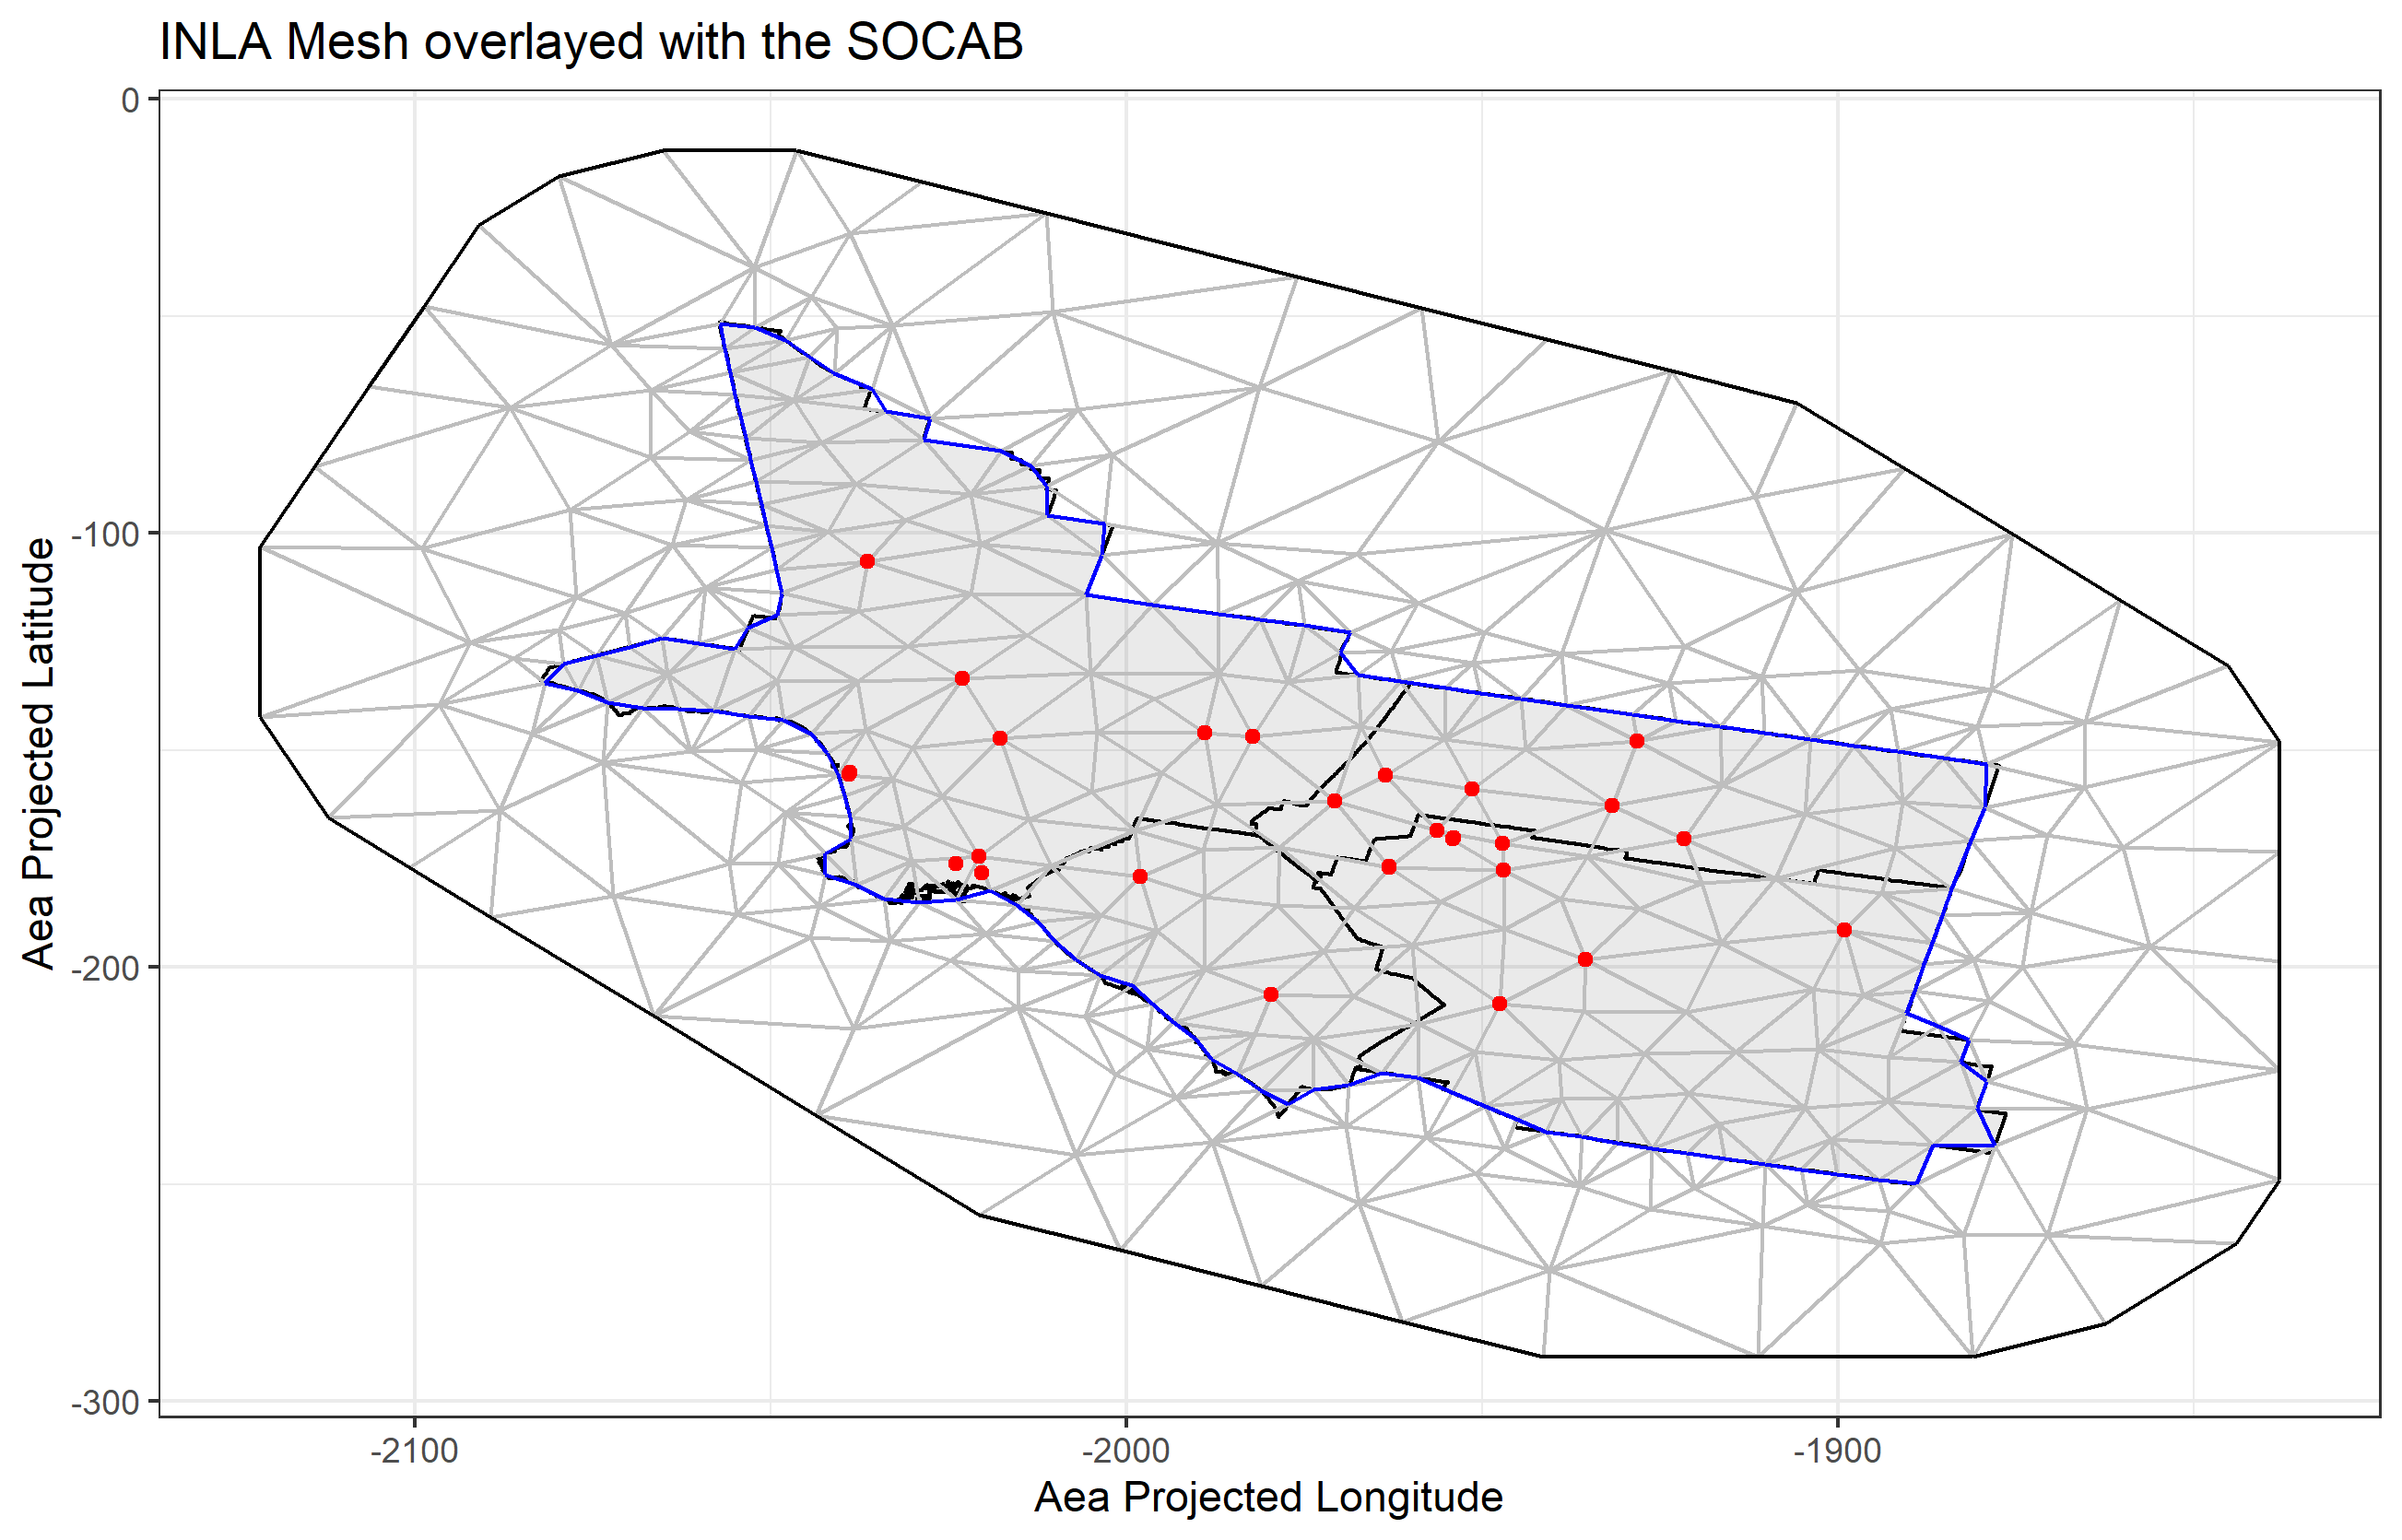
\includegraphics[width = \textwidth]{Figures/SOCAB_mesh.png}
	\caption{The mesh used for modelling, shown projected in the Albers projection.  The red dots are the locations of sites contributing data to the model.  The blue line is the boundary of the \ac{SOCAB} as defined in \ac{INLA}.  Under the blue line is a black line showing the actual legislated boundary.  There are a few sites close to the interior boundary, but no sites near the outer boundary.  By using sites as seed locations for the nodes, the problem of having multiple sites in one triangle was avoided.}
	\label{fig:SOCAB_mesh}
\end{figure}

\subsection{Mat\'{e}rn Parameters}
\label{subsec:maternparas}
The Mat\'{e}rn covariance function has several parameters that must be either estimated or fixed. These are the smoothness, $\kappa$, and the PC priors for the Range and Variance, as discussed in Section \ref{subsubsec:MaternIntro} and Section \ref{subsubsec:Priors}.

\subsubsection*{Smoothness, $\kappa$}
\label{subsubsec:smoothness}
As discussed earlier in Section \ref{subsubsec:MaternIntro} the Mat\'{e}rn's smoothness, $\kappa$, is fixed to make the choice of other parameters clear.  \cite{cameletti2011spatio} used $\kappa = 1$ for their Mat\'{e}rn function, we chose to use 1 as well.

\subsubsection*{Priors}
\label{subsubsec:priors}
Here are described the choices of \ac{PC} priors for the range, variance, and random walk used to generate the covariance function.

\subsubsection{Range}
\label{subsubsec:range}
The PC prior for the range is based upon the smallest value that is reasonably expected for the range.  This is done with the formula \ref{eq:PC_Matern_Range}.  The documentation for the PC prior suggests setting $p_r$ at 1\%. Table \ref{tab:Empirical_Range_Sill_Quantile} shows the range quantiles from the empirical variograms for each year, providing a guide for what value of $r$ to choose for the PC prior, we used $P(r < 6) = 0.01$.  

\begin{equation} \label{eq:PC_Matern_Range}
	P(r < r_0) = p_{r}.    
\end{equation} 

\begin{table}[ht]
	\centering
	\begin{tabular}{c||c|c}
		Quantile & Range (km) & Partial Sill \\
		\hline
		0\% & 4.34 & 0.00 \\
		1\% & 4.68 & 0.00 \\
		5\% & 6.17 & 0.00 \\
		10\% & 8.42 & 0.00 \\
		15\% & 9.37 & 0.012 \\
		25\% & 10.61 & 0.042 \\
		50\% & 20.55 & 0.066 \\
		75\% & 36.69 & 0.14 \\
		90\% & 349.42 & 1.65 \\
		95\% & 852.55 & 3.82 \\
		99\% & 2247.57 & 32.80 \\
		100\% & 2882.08 & 46.62 \\
		% SD Value &  0.00000000 & 0.00000000 & 0.00000000 & 0.00000000 & 0.01182547 & 0.04196286 & 0.06631998 & 0.13746604 & 1.64842843 & 3.81591636 & 32.79928596 & 46.62114477 
		% Range Value & 4.337855 & 4.679663 & 6.174913 & 8.417362 & 9.369826 & 10.612565 & 20.550440 & 36.693165 & 349.417833 & 852.549329 & 2247.574717 & 2882.078708
		
	\end{tabular}
	\caption{Empirical Quantiles of the range and partial sill of the 34 yearly Variograms using 1986 normalized log PM10. }
	\label{tab:Empirical_Range_Sill_Quantile}
\end{table}

\cite{cameletti2011spatio} Found range of 275 km and 1046 km for PM10 in Piedmont Valley

The \ac{EPA} describes spatial scale as follows:
\begin{quote}
	``Thus, the spatial scale of representativeness is described in terms of the physical dimensions of the air parcel nearest to a monitoring site throughout which actual pollutant concentrations are reasonably similar.''   \end{quote}
In CFR40-58, the \ac{PM10} sensors are defined as having a neighbourhood scale up to 4 km.  This implies that it would be physically impossible to resolve a range that is about 4 km or smaller.  With the information about the spatial scale of the sites from CFR40-58 and the combination of the empirical variograms of the \ac{SOCAB} and known range of \ac{PM10} from previous studies, it is reasonable to have $P(\rho < 3) = 0.01$. Implying it is unlikely that the range is smaller than 3 km.



\subsubsection*{Variance}
\label{subsubsec:variance}
The PC prior takes user input on the upper tail quantile and the probability of exceeding it as equation \ref{eq:PC_Matern_Stdev}.  Using the 34 years of empirical variograms, we get the quantiles shown in \ref{tab:Empirical_Range_Sill_Quantile} for the partial sill and then used $P(\sigma > 35) = 0.01$ as the prior on the partial sill.

\begin{equation}
	P(\sigma > \sigma_0) = p_{\sigma}    
\end{equation} \label{eq:PC_Matern_Stdev}

\subsubsection{Random Walk}
\label{subsubsec:ranwalk}
The \ac{RW} used in the full model was initiated with the same priors as the \ac{RW} performed during the data exploration, see Section \ref{subsubsec:RWexploration}.


\subsection{Choice of Covariance Structure}
\label{subsec:covstructchoice}
The final model was chosen from a range of options by comparing the DIC of models with different structures.  These structures were expanded from the core model of a single Mat\'{e}rn \ac{GRF} through the addition of an RW over time, an AR(1) process over time, and combinations of these.  \cite{cameletti2011spatio} used a Mat\'{e}rn field with an AR(1) process to account for shifts between observations periods.  This modelling was done with the full dataset.

Table \ref{tab:cov_str_DIC} summarizes the model results for these different covariance structures.  The models with smaller DIC are more attractive options for further modelling.  The model chosen is number 4, the combined \ac{GRF} and \ac{AR}(1) process, which is the same structure as that used by \cite{cameletti2011spatio}. 
\begin{table}[ht]
	\centering
	\begin{tabular}{l | c}
		Model Cov Structure & DIC  \\
		\hline
		Mat\'{e}rn & 2.385e+02  \\
		Mat\'{e}rn and RW1 & -8.385e+02 \\
		Mat\'{e}rn and RW2 & -8.349e+02 \\
		Mat\'{e}rn, RW1, and AR1 & -9.173e+02 \\
		Mat\'{e}rn, RW2, and AR1 & -8.969e+02
		
	\end{tabular}
	\caption{The data used is the log of the normalized data as shown in equation \ref{eq:log_transform}.  The covariance structures are listed in order of increasing complexity. \ac{RW}(1) is the smoothing that describes the transition of the overall mean from one year to the next.  \ac{GRF} is the Mat\'{e}rn function taken as an overall mean for the whole year.  }
	\label{tab:cov_str_DIC}
\end{table}

The equation describing the final model is as follows:

\begin{subequations}
	\begin{equation}
		Z(s,t) = \beta_0 + \Delta y_t + y(s,t) + \epsilon(s,t)
	\end{equation}
	\begin{equation}
		\Delta y_t = y_t - y_{t-1}
	\end{equation}
	\begin{align}
		y(s,1) &\sim N \left(0, \frac{\sigma^2_w}{(1-a^2)} \right) &, |a| < 1 \\
		y(s,t) &= ay(s,t-1) + w(s,t) &, t>1
	\end{align}
	\begin{equation}
		cov(w(s,t), w(s,t')) = 
		\begin{cases}
			0 \text{ if } t \neq t' \ , \\
			\sigma^2_w \gamma(u) \text{ otherwise, }  \gamma(u) \sim \text{Mat\'{e}rn.}
		\end{cases}
	\end{equation}
\end{subequations}

\subsubsection*{Final Model} \label{seq:finalModel}

Table \ref{tab:model_INLA_full} gives the results of the final model, performed on a randomly selected 90\% of the data, holding the other 10\% for validation, see Section \ref{subsec:validation} for details.  The model has a \ac{RW}1 structure portraying the trend over time, a Mat\'{e}rn covariance function describing the spatial structure and an \ac{AR}(1) function describing how that structure changes over time.

\begin{table}[ht]
	\centering
	\begin{tabular}{l|c|c}
		& Value & SD  \\
		\hline
		WAIC & -7.958e+02   & \\
		DIC & -8.022e+02 & \\
		Intercept & -0.0005082417 & 31.58598  \\
		RW1 & [-1.36122, -0.114299] & [31.5861, 31.5861] \\
		Mat\'{e}rn & [-0.408501, 0.58749] & [0.0812534, 0.349748] \\
		Hyperpar Gaussian Prec. & 73.6006189  &  2.811640470 \\
		Hyperpar RW1 Prec & 60.1411588 & 7.967774153 \\ 
		Hyperpar Mat\'{e}rn Range & 23.8506006 & 6.017936799 \\
		Hyperpar Mat\'{e}rn Stdv & 0.2729190 & 0.023497256 \\
		AR(1) rho & 0.9923009 & 0.001750823 
	\end{tabular}
	\caption{Summary results of model that has RW1 over the years, a Mat\'{e}rn spatial process and an AR(1) term.   The RW1 and Mat\'{e}rn are random variables and so take on a unique value at each site. }
	\label{tab:model_INLA_full}
\end{table}

The following code is how the model was constructed in R with \lstinline{INLABru}.
\begin{lstlisting}
	cmp.Matern.RW1.AR1.PM10.subsample = log.Arthmt.M ~ 
	Intercept + trend(map = year, model = ``rw1'', 
	constr = FALSE, n = n_year, hyper = rw_pc_prior) +
	myspde(map = coordinates, group = year,\ngroup = n.year,
	model = inla.spde2.pcMatern(mesh1, alpha = Matern_alpha,
	prior.range = Matern_pc_prior_range,prior.sigma = 
	Matern_pc_prior_sigma),mesh = mesh1,control.group=list(model=``ar1''))
	bru.Matern.RW1.AR1.PM10.subsample = bru(cmp.Matern.RW1.AR1.PM10.subsample,             
	family = ``gaussian'', data= PM10.INLA.data.aea.subsample.SOCAB)
\end{lstlisting}


\subsection{Prediction and Validation} \label{subsec:validation}
The \ac{PM10} surface for each discrete year was interpolated using the model described in Section \ref{seq:finalModel}.  This surface was used for subsequent preferential sampling testing as well as model validation.  The prediction was performed on a grid of pixels covering the \ac{SOCAB} with each pixel approximately 2 km square as defined by the Lambert projection.  After predicting the surface, the results were used to examine whether the model did a ``good job'' of describing the known observations.

\subsubsection*{Withholding 10\% of Data}
\label{subsubsec:withholding}.
Model validation was done while holding out a randomly selected 10\% of the data.  The sites and years that were withheld can be seen in Figure \ref{fig:validate_dotplot}.  The model was then used to predict that 10\% and the results compared to the actual values.  The difference between the prediction and the actual observed value can be seen in Figures \ref{fig:validate_delta_mean} and \ref{fig:validate_delta_site}.   This is a basic but easy-to-implement method that is not computationally intensive.

It is concerning that Figure \ref{fig:validate_delta_mean} shows such a high percentage of sites whose prediction interval does not contain the actual observed value.  Theoretically, only 5\% of the validations should not contain the actual value within the 95\% prediction interval.  The variance could be underestimated, or the model could be too smooth.

Figure \ref{fig:validate_delta_site} suggests that there isn't any obvious prediction problem at individual sites, so maybe it is the variance that is too small.


\begin{figure}[ht]
	\centering
	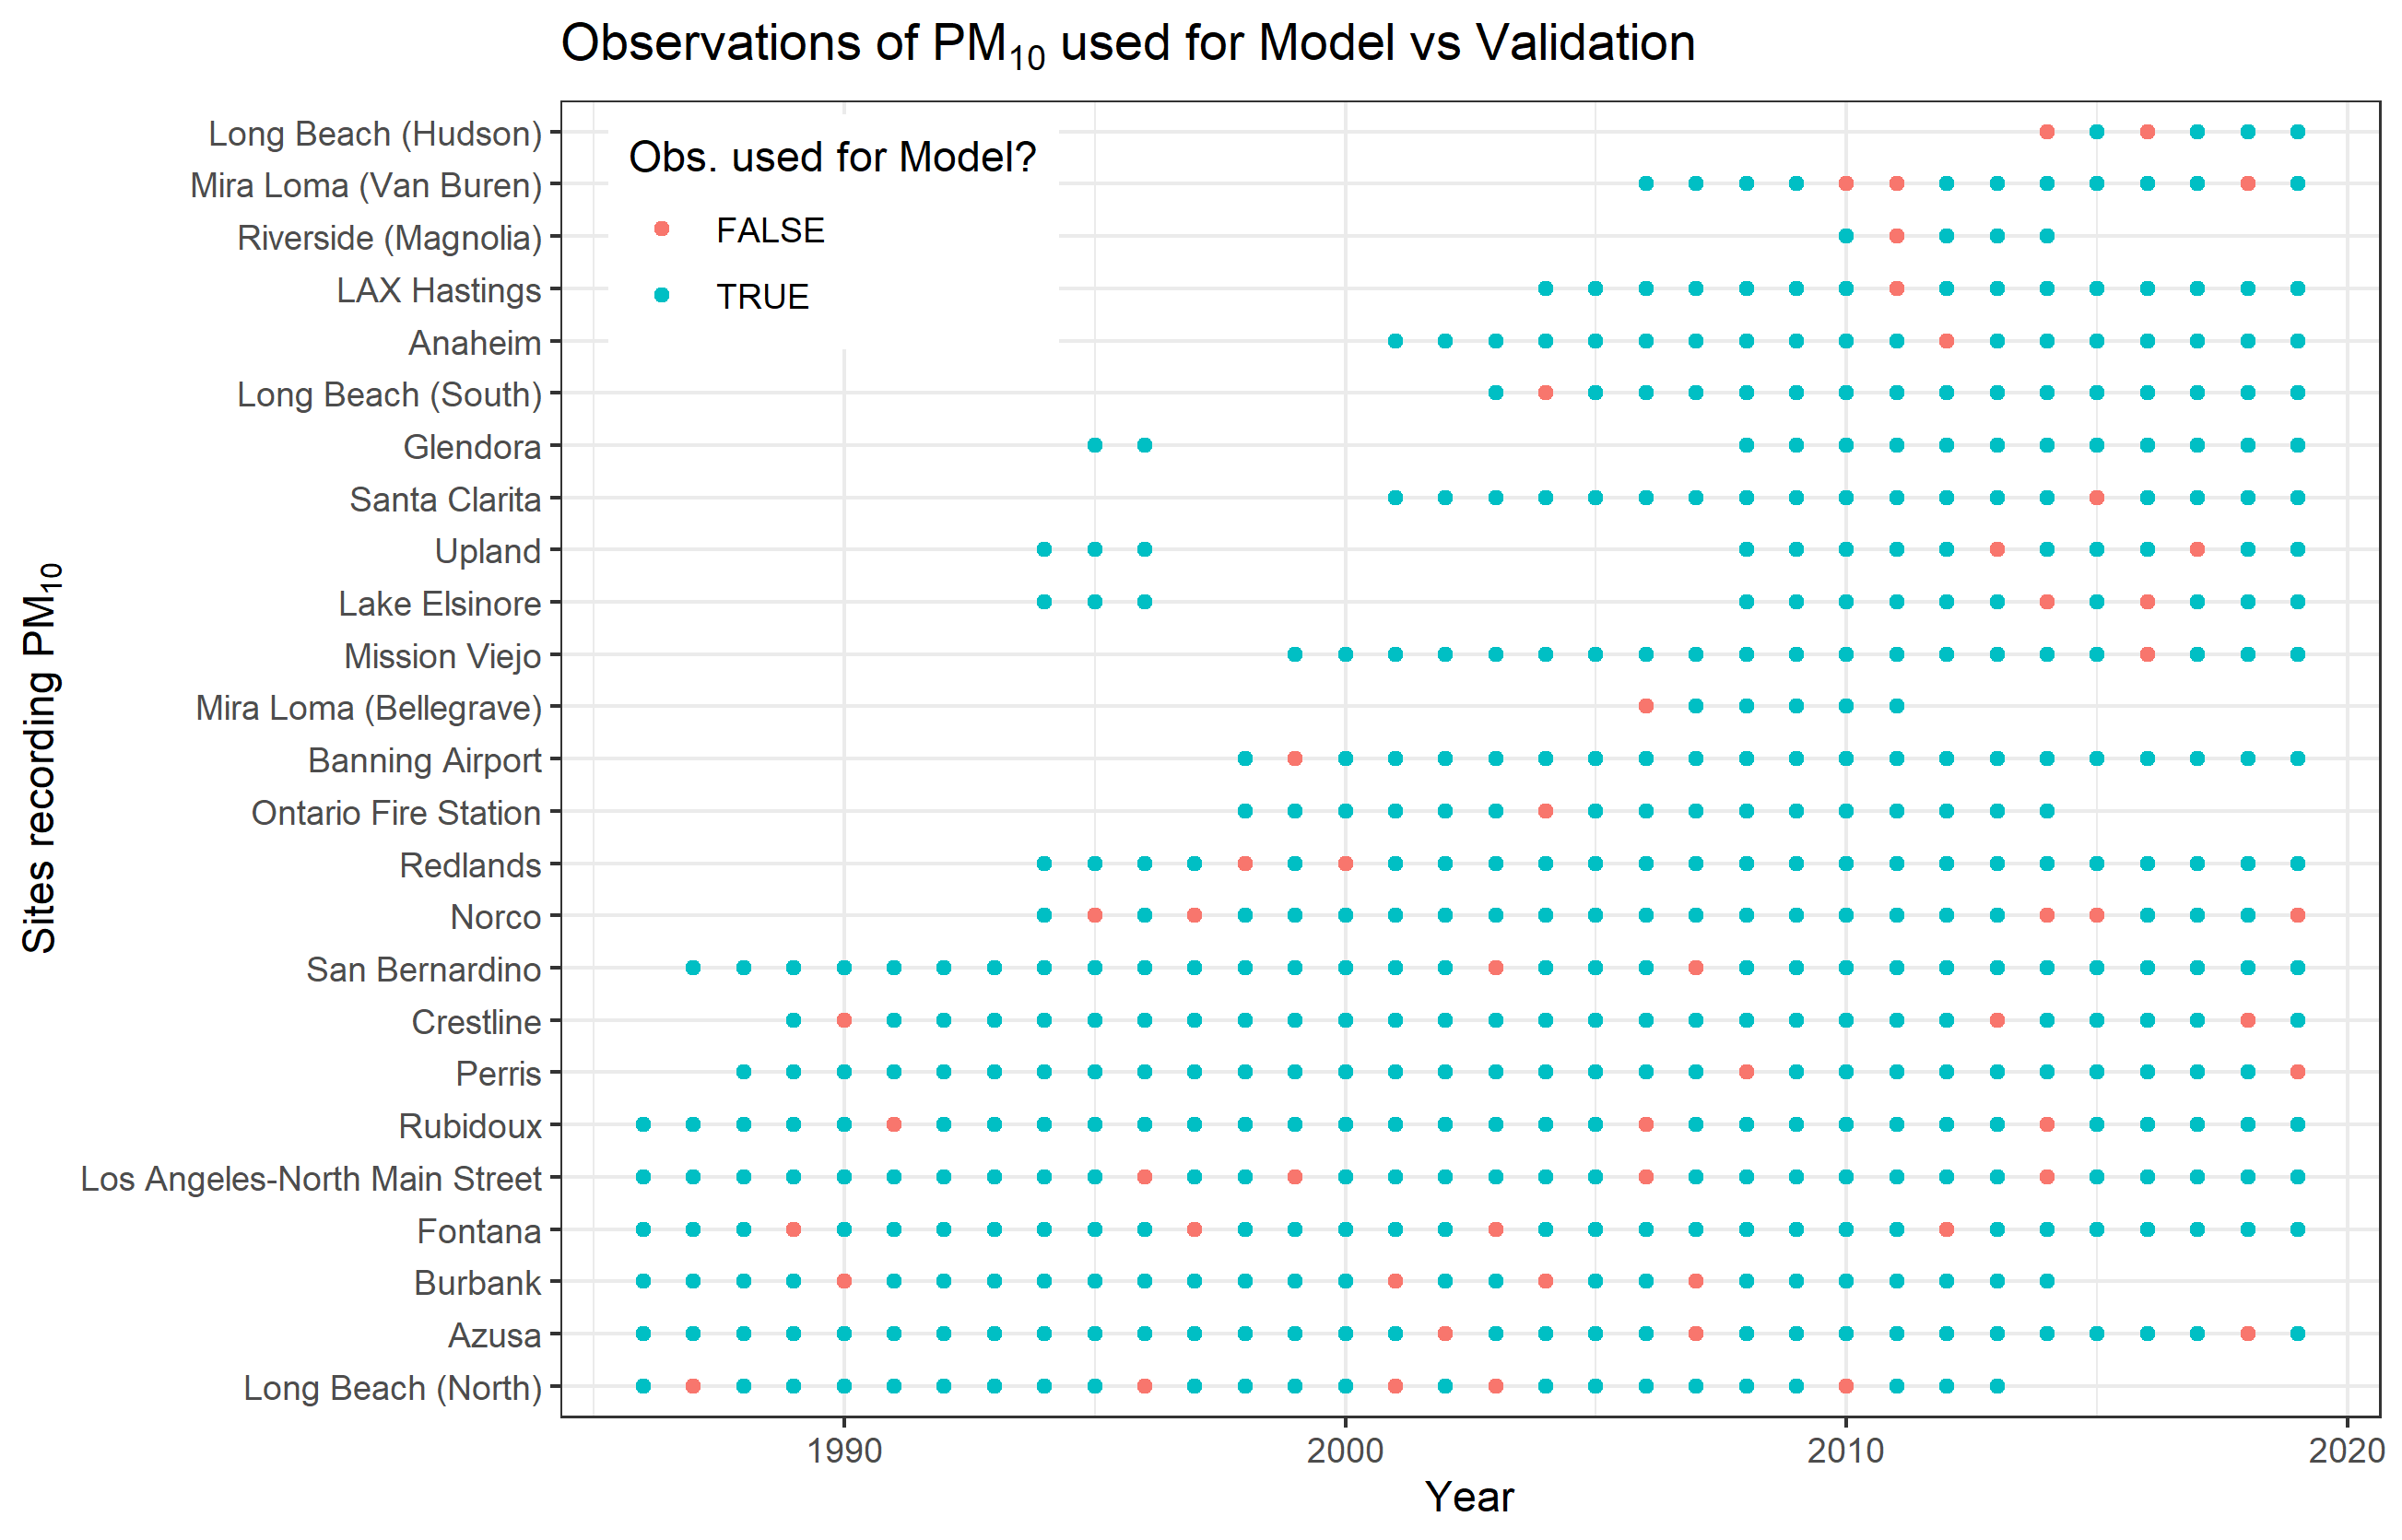
\includegraphics[width = \textwidth]{Figures/Validation/validate_dotplot.png}
	\caption{The red dots are observations that were kept out of the model for use in future validation.  Eighty (ten percent) of the 822 total observations were held back, chosen at random}
	\label{fig:validate_dotplot}
\end{figure}

\begin{figure}[ht]
	\centering
	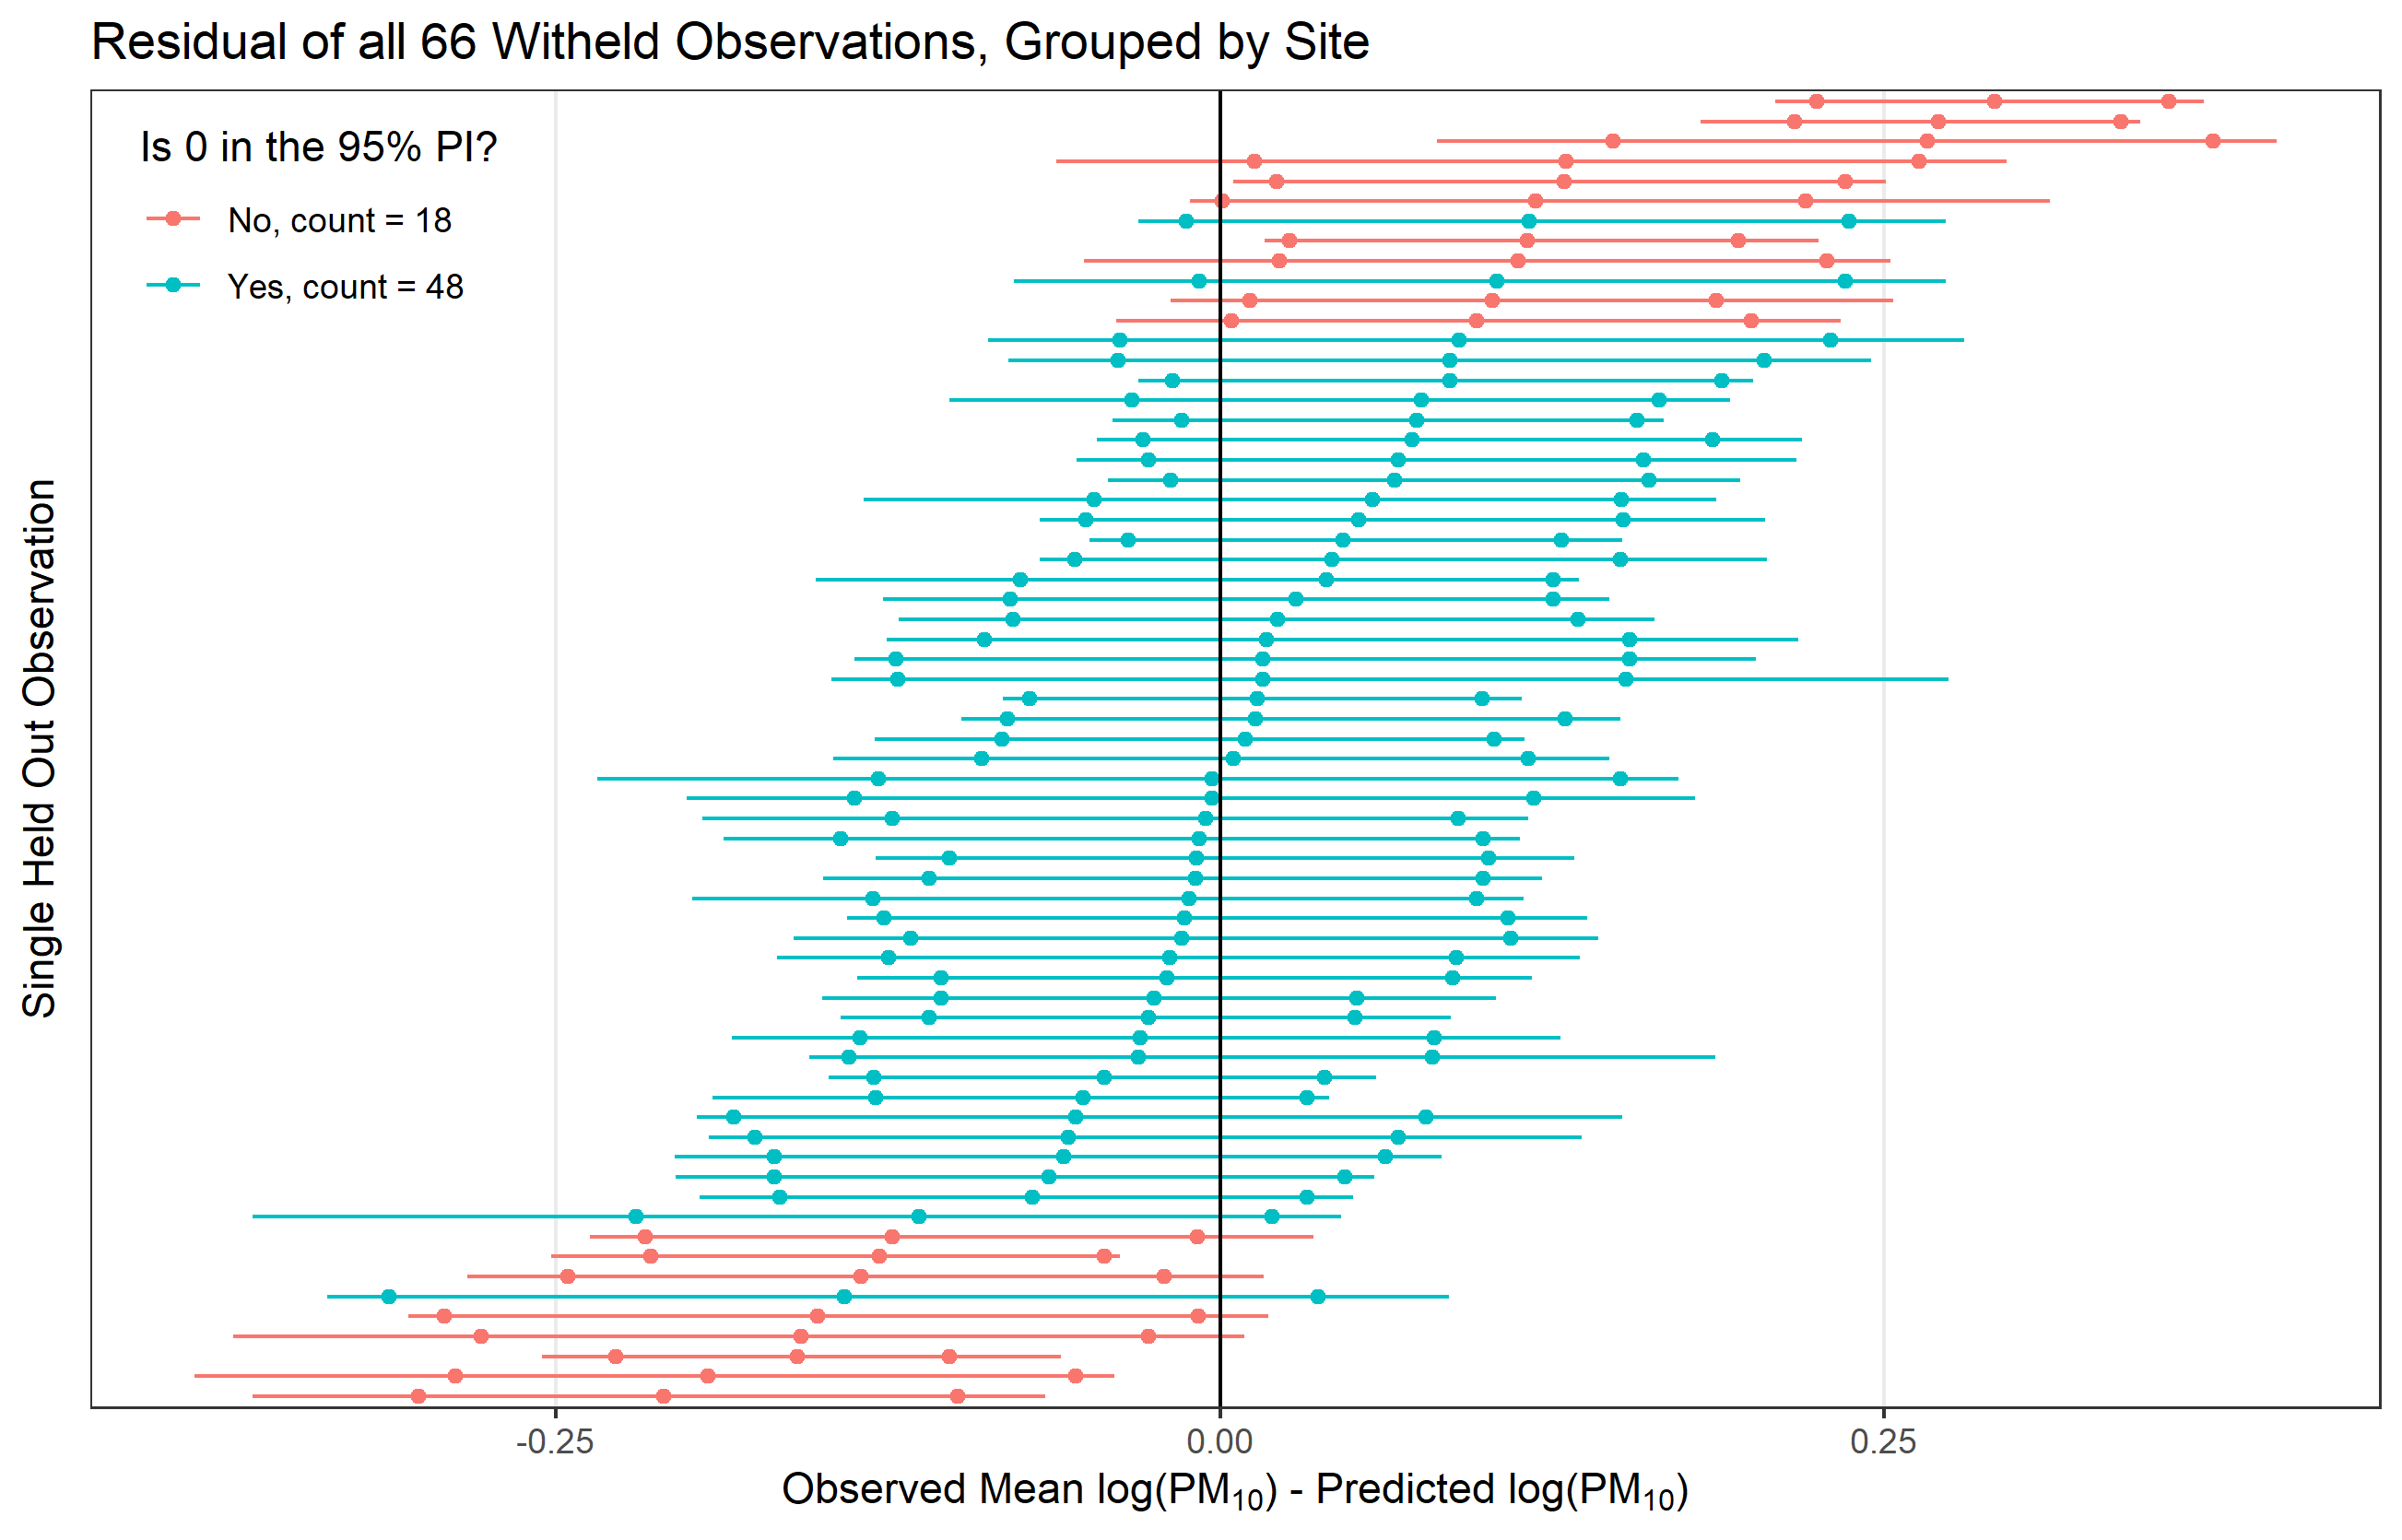
\includegraphics[width = \textwidth]{Figures/Validation/validate_delta_mean.png}
	\caption{This shows the posterior distribution of the withheld observations, centred at 0 by subtracting them from the observed observations.  For each site, the central point is the posterior mean, the left and right points are the posterior 0.025 and 0.975 percentiles respectively, and the line goes from the smallest to the largest value in the 100 samples from the posterior.  It is concerning that 35\% of the validation points don't have the observed value within the 95\% prediction interval, which suggests that some parts of the model could be improved.}
	\label{fig:validate_delta_mean}
\end{figure}

\begin{figure}[ht]
	\centering
	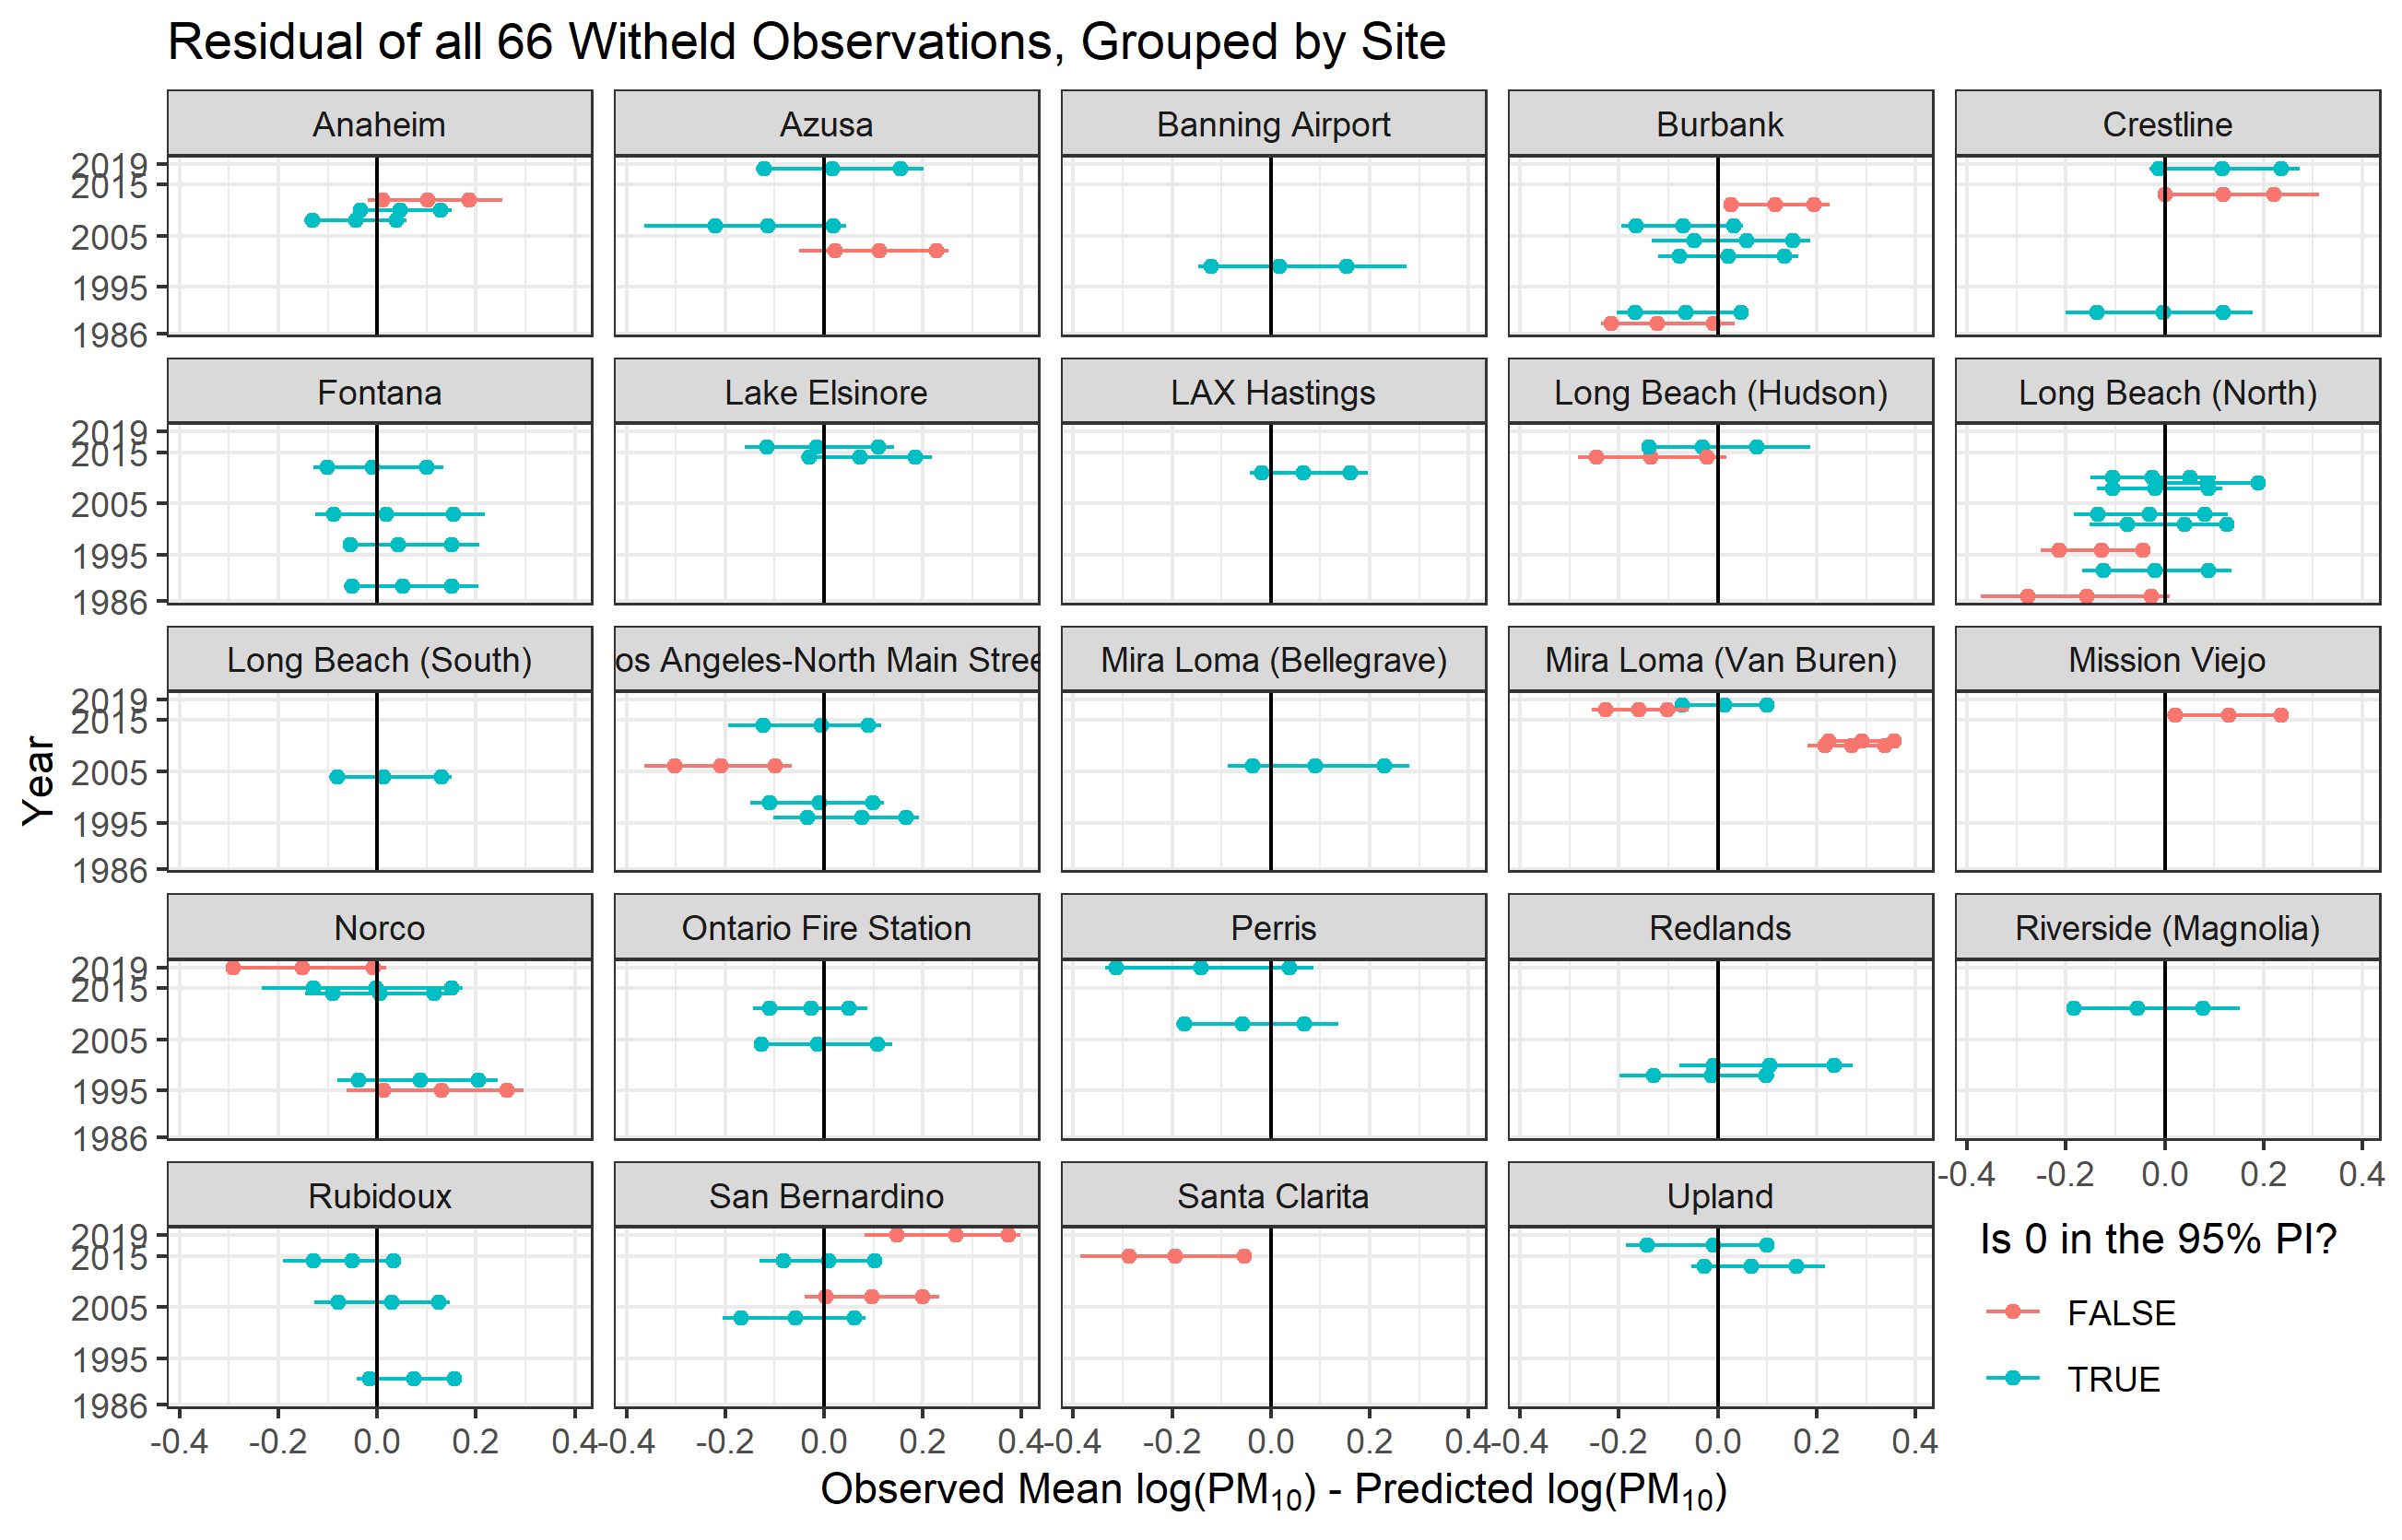
\includegraphics[width = \textwidth]{Figures/Validation/validate_delta_site.png}
	\caption{Here the posterior distributions shown in the previous figure are split up by site and by year in an attempt to see any patterns suggesting where the model could be improved.  It looks like sites have more heterogeneity in the distribution of out-of-bounds predictions than years, so perhaps the spatial covariance function needs tweaking.}
	\label{fig:validate_delta_site}
\end{figure}


%\include{06_Preferential_Sampling}
\section{Preferential Sampling}
\label{sec:prefsamp}

As discussed in Section \ref{subsec:PreferentialSampling}, \ac{PS} results in sampling sites that have a stochastic dependence upon the latent field of interest and results in a biased estimation of the true field.  This chapter presents evidence  \ac{PS} found in the course of this project.

The test for preferential sampling is done by comparing the location of all sites to simulated sites sampled on the pollutant field, a field calculated from all the sites.  To that end, after the validation modelling that held back 10\% of the data, the same model using all the data was run.

\subsection{Governmental Acknowledgement of Preferential Sampling} \label{subsec:govPrefSamp}
The first and perhaps most clear-cut evidence for \ac{PS} are direct statements from the agencies responsible for site selection, the \ac{SCAQMD} and \ac{EPA}.  In their five-year reports, the \ac{SCAQMD} describes some of how the monitoring locations are distributed.  On page 63 of the 2010 \ac{SCAQMD} 5-year report and page 83 of the 2015 version is the following statement:
\begin{quote}
	``Real-time monitors, for the most part, are clustered in the high concentration areas...''  ``Real-time \ac{PM10} monitors also support ongoing health studies in the region.''    
\end{quote} \cite{CASCAQMD:2010}, \cite{CASCAQMD:2015}, \cite{AQMNP:2019}
Site clustering is one way that \ac{PS} is described, and its presence is used by \cite{watson2020} as an indicator for the presence of \ac{PS}. 

\begin{quote}
	``Though the current PM 10 network is relatively stable, monitoring agencies may  continue divesting of some of the PM10 monitoring stations where concentration levels are low relative to the NAAQS.''
\end{quote} \cite{EPA:IntegratedReview}
This divesting of low-concentration sites from the network is similar behaviour to that found in the UK for black smoke \citep{zidek2010monitoring}.

\subsection{Four Site Categories}\label{sec:4sitecategories}
In Figures \ref{fig:site_timing_trace-Added}, \ref{fig:site_timing_trace-Continuous}, and \ref{fig:site_timing_trace-Removed} We demonstrated the first sign of preferential sampling in the data, by examining the traces of sites grouped by when they entered and left the network.  Sites were split by a 2-by-2 table based on whether a site was A) present at the start of the network or B) still monitoring at the end of the network (see table \ref{tab:2X2_site_category}).

\begin{table}[ht]
	\centering
	\begin{tabular}{| c c | c c |}
		\hline
		\multirow{2}{*}{} & {} & \multicolumn{2}{c}{Present in 1986} \\
		& {} & Yes & No \\
		\hline 
		\multirow{2}{*}{Present in 2019} & Yes & Continuous (many) & Added (many) \\
		& No & Removed (2 sites) & Added then removed (3 sites)   \\
		\hline
	\end{tabular}
	\caption{Naming conventions for sites categorized according to the two-way table made by whether the site is A) Present in the network in 1986, and B) Present in the network in 2019.}
	\label{tab:2X2_site_category}
\end{table}

Calling back to those three figures, the ``Continuous'' and ``Added then Removed'' sites have very similar overall means, an increase compared to the overall mean of all sites.  In contrast, the ``Removed'' and ``Added'' sites have similar means that are lower compared to the overall mean.
This pattern could be a result of preferential sampling early (starting biased high, then corrected by adding low pollution sites later) or late (ending biased low, the mean dragged down by the sites added later). Alternatively, a change in the pollution field's distribution could explain this; if the tail shifts and drags the mean over time.  However, the box plots of each year do not seem to support that explanation,
as they stay roughly symmetrical throughout.

Table \ref{tab:model_INLA_4site_Retention} shows the result of including those four categories as fixed effects in the model

\begin{table}[ht]
	\centering
	\begin{tabular}{l|c|c}
		& Value & SD  \\
		\hline
		WAIC & -9.532e2 & \\
		DIC & -9.645e2 & \\
		Intercept & -0.0004295981  & 31.59055710 \\
		Continuous & 0.0094430558  & 0.12665671   \\
		Removed & -0.2024973929   & 0.10773814   \\
		Temporary & -0.2746064961   & 0.04417141\\
		RW2 & [-1.38555, -0.106361] & [31.5907, 31.5908] \\
		Mat\'{e}rn & [-0.394883, 0.70015] & [0.107131, 0.427265] \\
		Hyperpar Gaussian Prec. & 82.1063483 & 5.363589751  \\
		Hyperpar RW2 Prec. & 30.2078731   &  8.969724584 \\
		Hyperpar Mat\'{e}rn Range & 28.0537004  & 11.325932812  \\
		Hyperpar Mat\'{e}rn Stdv & 0.2980578  & 0.043042302   \\
		Hyperpar AR(1) rho & 0.9948262   & 0.001907155  
	\end{tabular}
	\caption{Including fixed effects for the 4 site retention category }
	\label{tab:model_INLA_4site_Retention}
\end{table}

%Statistic comparing group means, e.g. ANOVA?
%Statistic comparing distribution, e.g. nonparametric something or other?


\subsection{\texttt{PStestR}: A Preferential Sampling Package}
\label{subsec:prefsamppkg}

As described in Section \ref{subsubsec:WatsonPrefSample}, \citet{watson2020} proposed a theory to detect preferential sampling.  They also provide an R package called \texttt{PStestR} to implement the test, which is used below.

\subsubsection*{Implementation in \texttt{PStestR}}
\label{subsubsec:implementation}
Having obtained a predicted pollutant surface and knowing the location of sites, the package calculates the mean of the \gls{k} nearest neighbours at each site and correlates that with the estimated concentration of the pollutant. The same result is produced for many Monte Carlo samples of possible sites over the whole network area.
The package described in \cite{watson2020} can be used under two paradigms. 
\begin{enumerate}
	\item The number of nearest neighbours to use is known.
	\item The number of nearest neighbours is uncertain, and testing a range of options is part of the research question.
\end{enumerate}
In the first case, a single test is performed comparing the known sites to the distribution of the Monty Carlo samples.  In the second case, a multiple comparison test is implemented with a comparison for each value of \gls{k}, the number of nearest neighbours used.  \texttt{PStestR} then provides the following outputs:
\begin{itemize}
	\item Test Rho:  The calculated Spearman's Rho for the network during each year.
	\item Empirical P-Value:  Compares the Test Rho for the actual network to the distribution from the Monte Carlo simulation.
\end{itemize}

\subsubsection*{Tuning Parameters}
\label{subsubsec:tuneparameters}
\texttt{PStestR} has several parameters that can be adjusted to affect the simulation and test.  Here we describe those parameters and what we chose to use.

\begin{itemize}
	\item Number of Nearest Neighbors, \gls{k}:
	As described earlier, the number of nearest neighbours included in the test can be tuned to improve the power of the overall test at the cost of precision.  Looking at the points showing site locations in fig \ref{fig:site_dotplot}, the largest cluster seems to be about 3.  So we set $k = 3$.  
	
	\item Number of Monte Carlo Samples:
	Increasing the number of Monte Carlo samples improves the posterior's precision at the cost of computational time.  An M of 1000 is large enough to be reasonable while still being manageable by the computer on which this analysis was performed.
	\item Year:
	Each year is not independent of the others, but each test on a year will assume that it is.  To avoid multiple comparisons, it is necessary to choose one year to test.  We chose 2019 because it will show the current state of the network.
	
\end{itemize}


\subsection{Results of Test}
\label{subsec:testresults}

\subsubsection*{Result of Test for 2019}
\label{subsubsec:test2019}


The network in 2019 has a correlation of -0.822 and an Empirical P-value of 0.00300. 
This correlation is very close to -1 and the P-value implies that the observed network of sites would be very unlikely to be chosen in a sampling regime that is not stochastically dependent upon the pollutant field.  

Figure \ref{fig:MCMC_hist} shows the distribution of the test Rho for each of the MCMC samples and the position on that distribution of the test Rho for the actual network during 2019.
\begin{figure}
	\centering
	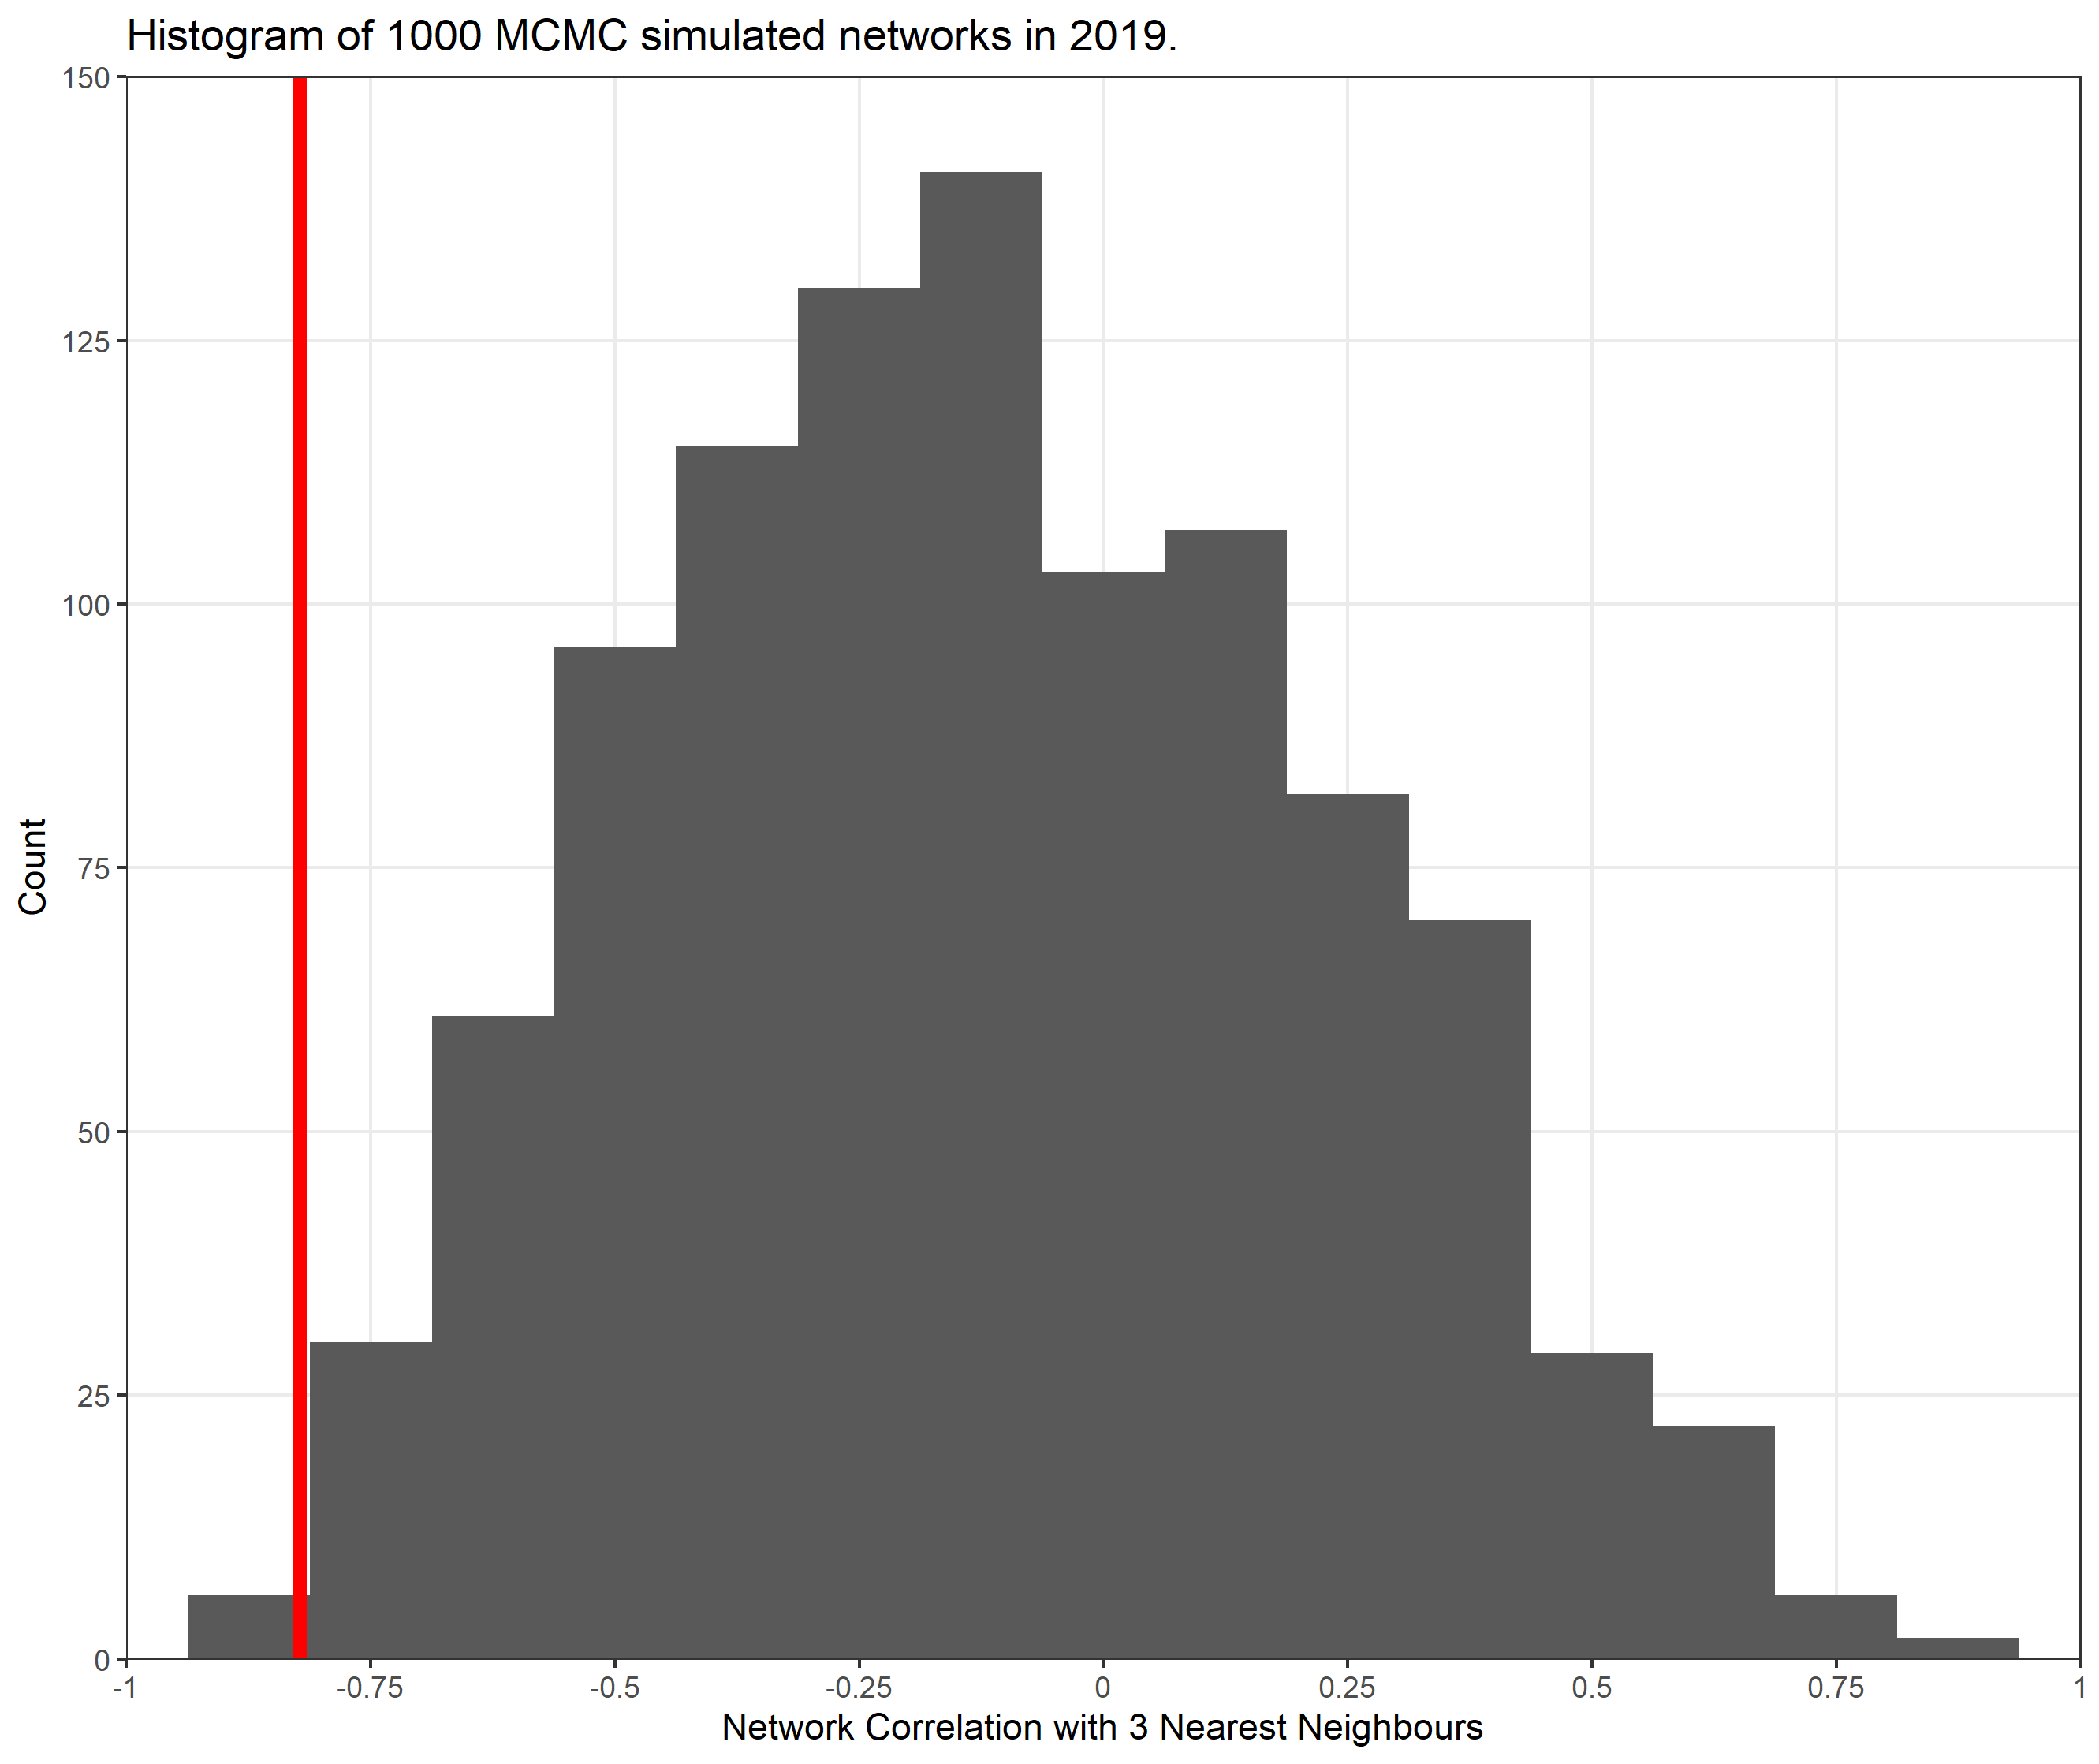
\includegraphics[width = \textwidth]{Figures/PreferentialSampling/PrefSmpl_nonn3_hist_MCMC_rho.png}
	\caption{Histogram of sampled network Correlation of 1000 MCMC samples showing their empirical distribution.  The red line shows where the observed correlation lies in relation to the samples.}
	\label{fig:MCMC_hist}
\end{figure}

\subsubsection*{Time Series of Test Score} \label{subsubsec:TestScoreTimeSeries}
Despite knowing there is a lack of independence between years, we chose to assess the data as a time series.  What follows is a more qualitative exploration rather than a quantitative result.

Before 1994 the network did not have enough sites to produce a result from the \texttt{PStestR} algorithm.  However, except for 1997, from 1994 to the present there are enough sites for a correlation score.  

Figure \ref{fig:PS_site_counts_test_rho} shows that each year has a negative correlation score, implying preferential sampling for locations with a higher concentration of \ac{PM10}.  In addition, the Test Rho's time series in the bottom half of Figure \ref{fig:PS_site_counts_test_rho} shows a decrease in time, which would imply an increase in preferential sampling from earlier to later dates.  On the other hand, the ``trend'' could easily result from a stationary time series. 

To examine whether the scores can be explained by a stationary time series, ACF and PACF plots of the Test Rho (Figure \ref{fig:test_rho_acf_pacf}) were produced.  There are two ways of handling the missing value for 1997 while calculating the ACF and PACF:  (1) interpolate the missing year; (2) cut out the time series before the missing year.  We chose option (1) and so interpolated the missing year's Test Rho by using the mean of 1996 and 1998.  Figure \ref{fig:test_rho_acf_pacf} suggests the Test Rho time series is stationary, with a possible AR(1) process.  

\begin{figure}
	\centering
	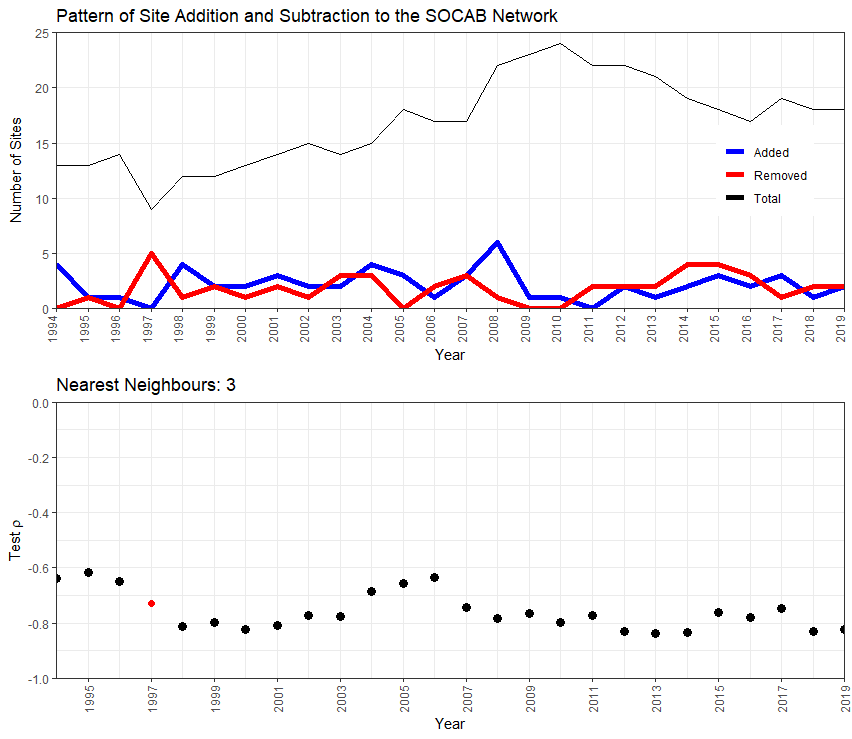
\includegraphics[width = 
	\textwidth]{Figures/PreferentialSampling/PrefSmpl_nonn3combine_siteCounts_TestRho.png}
	\caption{Top:  Counts of sites in the network for each year.  Total sites are in black, the number of sites that were removed compared to the previous year is in red, and several sites that were added compared to the previous year are in blue. 
		Bottom: Test $\rho$ (Spearman's Rank Correlation) for the three nearest neighbours.  A negative correlation implies a bias towards high-concentration monitoring. 1997 had too few sites to calculate a score and is interpolated as the mean of 1996 and 1998 scores (red dot).}
	%}
\label{fig:PS_site_counts_test_rho}
\end{figure}

\begin{figure}
\centering
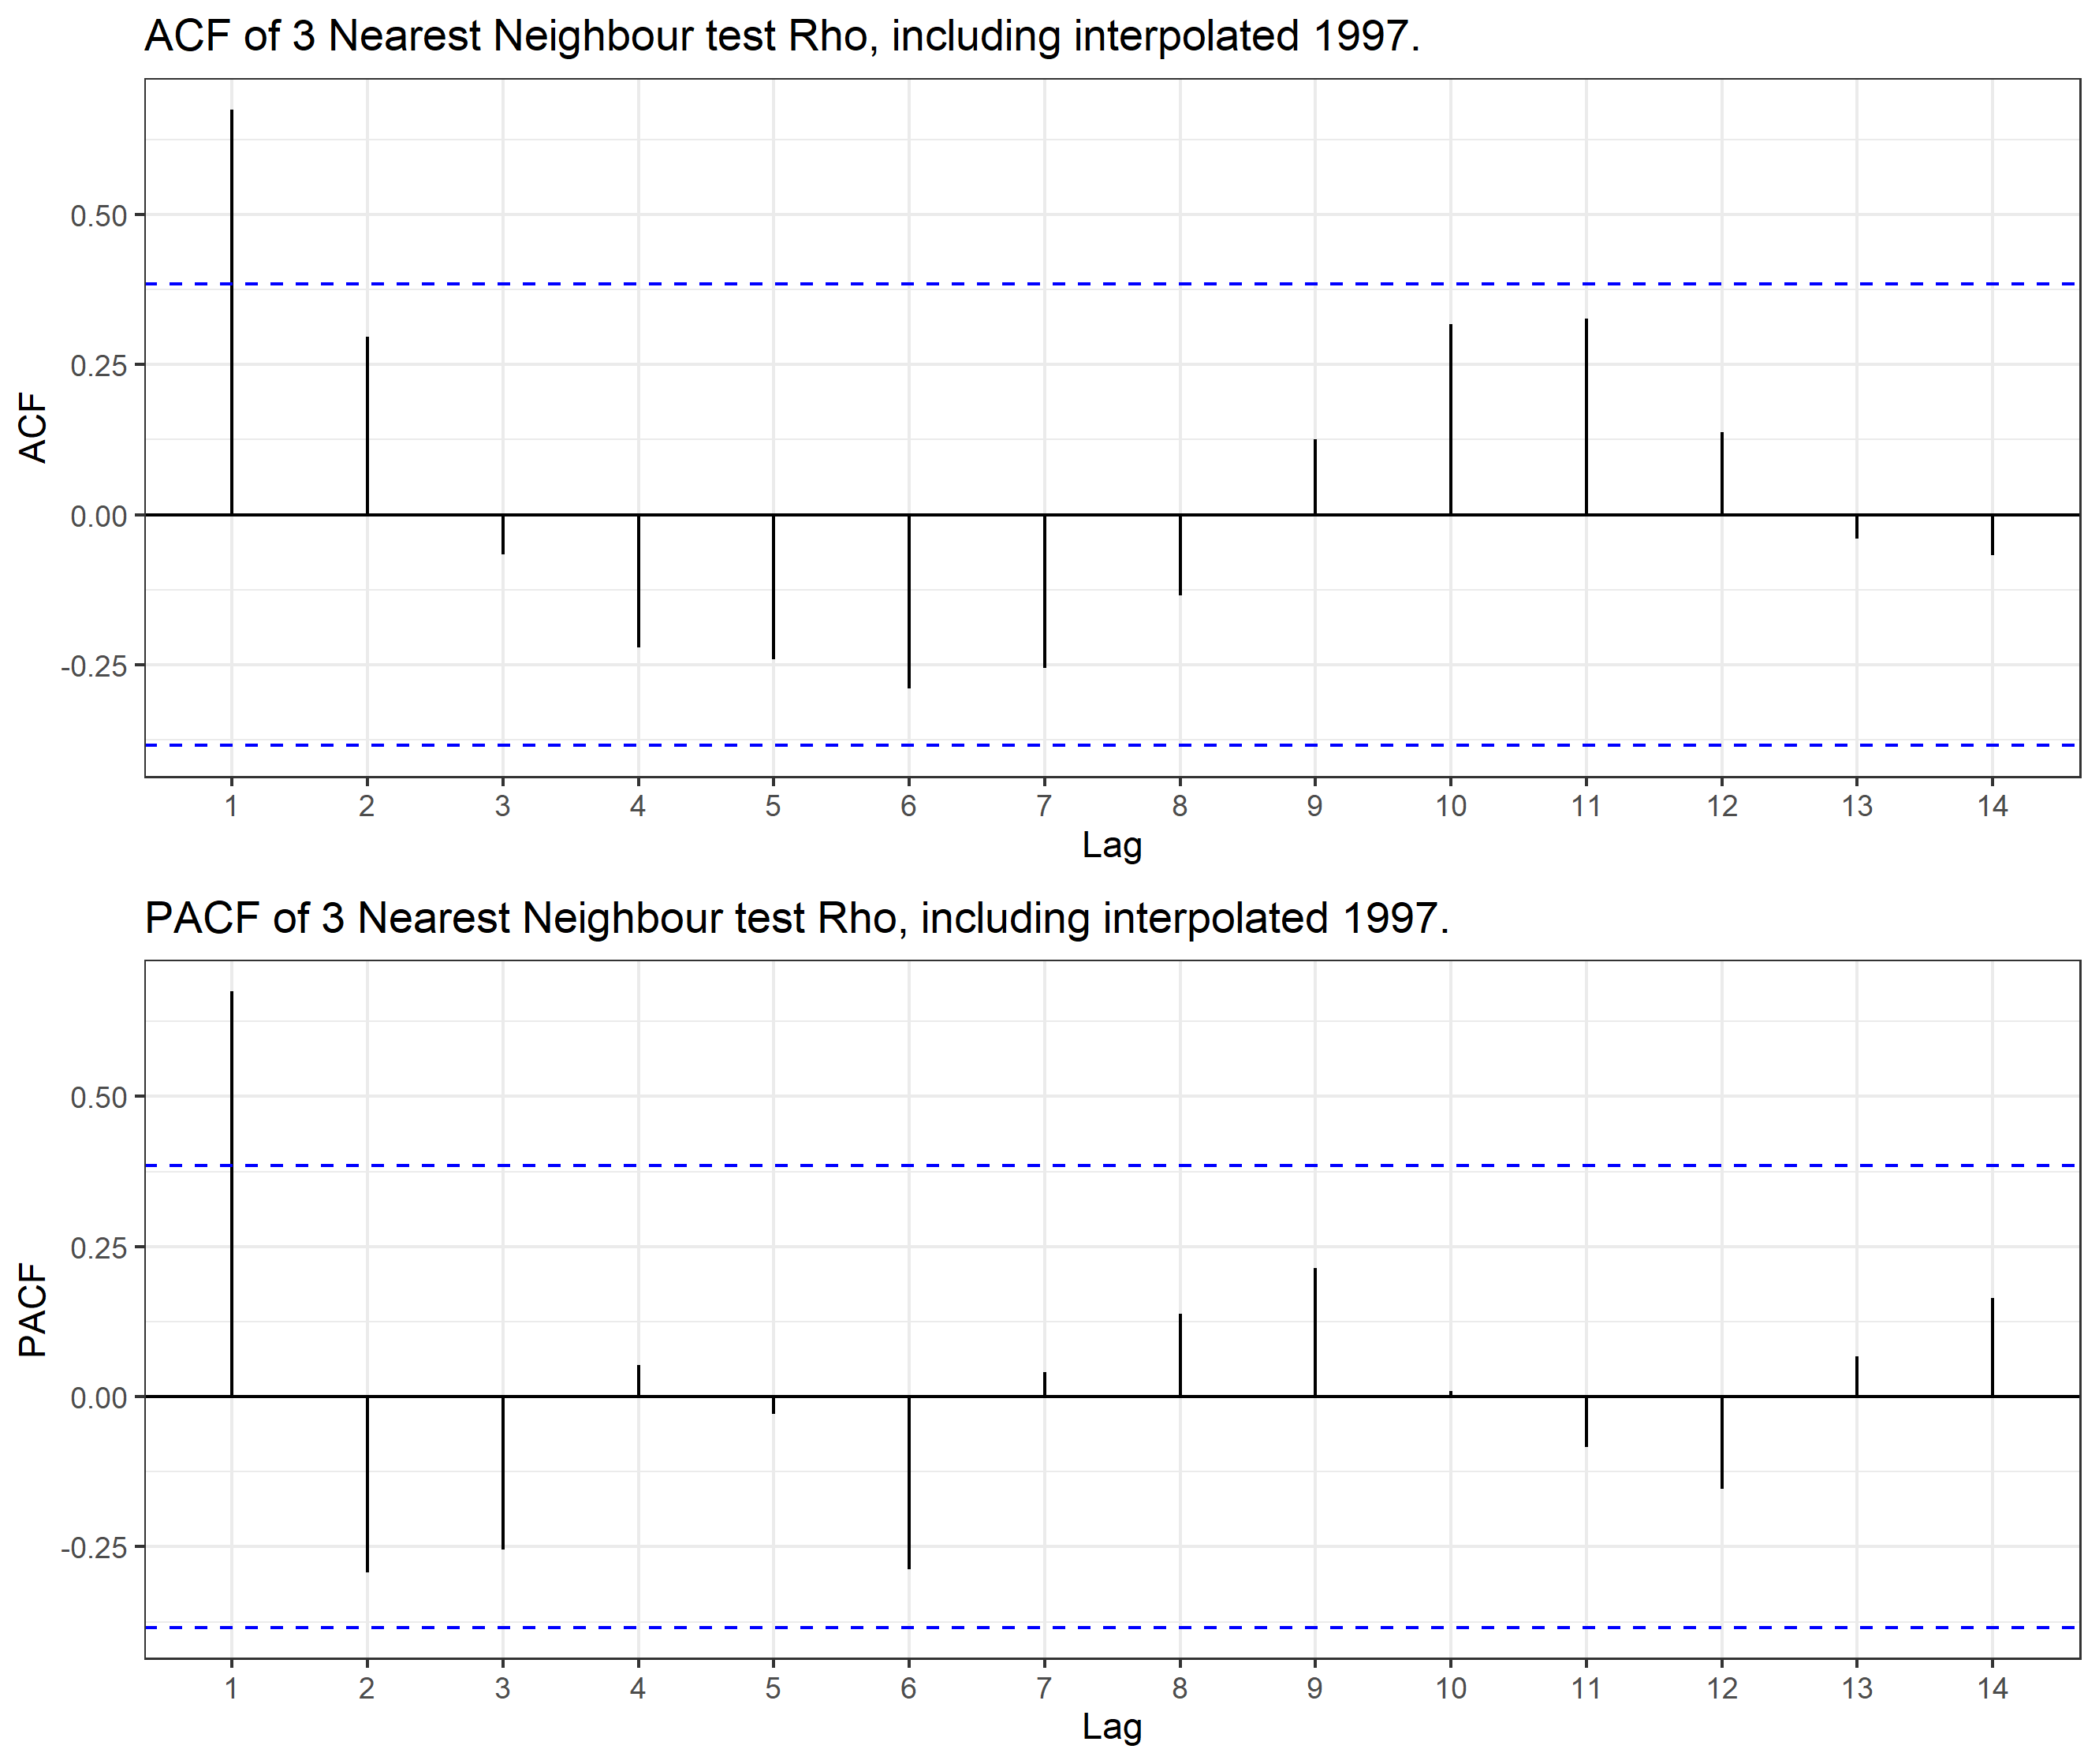
\includegraphics[width = \textwidth]{Figures/PreferentialSampling/test_rho_acf_pacf_interp1997.png}
\caption{An examination of the autocorrelation of the nearest neighbours.  With both quickly decaying, it seems unlikely that there is nonstationarity in the time series.   Note that since sites carry over from year to year, each year's correlation is not an independent observation.  This uses the interpolated value for 1997 as part of the time series.  With the spike in ACF and PACE at lag 1, the smooth decay in the ACF, and the sharp drop-off in the PACF, an AR(1) process seems a plausible model choice.}
\label{fig:test_rho_acf_pacf}
\end{figure}

The final issue we investigated is whether a  relationship between the Test Rho and the addition or removal of sides from the network exists, ie the dots and the red and blue lines in Figure \ref{fig:PS_site_counts_test_rho}.  This could be another indicator of administrative choices resulting in preferential sampling over time as the network evolves.  Spearman's correlation between the time series test scores and the two-time series of network site changes was used.   One correlation with the interpolated point included was done, and one with that year removed from the site counts.

\begin{table}[ht]
\centering
\begin{tabular}{c|c|c}
	
	&  Interpolated 1997 & 1997 Absent\\
	\hline
	Number of Added Sites & 0.02921195 & 0.09615902 \\
	Number of Removed Sites & -0.1937513 & -0.2670485
\end{tabular}
\caption{Spearman's Rho between the network's Test Rho and the number of sites added or removed from the network compared to the previous year.}
\label{tab:testRho_siteChange}
\end{table}
%TestRho with 1997 ~ NumAdded [1] 0.02921195
%TestRho without 1997 ~ NumAdded [1] 0.09615902

%TestRho with 1997 ~ NumLost [1] -0.1937513
%TestRho without 1997 ~ NumLost [1] -0.2670485

Table \ref{tab:testRho_siteChange} shows the results of the correlation.  Adding sites seems to have very little correlation with the network's Test Rho over the years of monitoring.  Site removal has a stronger correlation, but still not much.